\documentclass[man]{apa7}

\input{includes/preamble_common}
\input{includes/preamble_apa7}


	\title{Desarrollo de un sistema de software basado en patrones de diseño y buenas prácticas de programación}
\shorttitle{Desarrollo de sistema de software}
\authorsnames{July Ramos}
\authorsaffiliations{SENA - Servicio Nacional de Aprendizaje, Colombia}
\authornote{Correspondencia: july_ramos@soy.sena.edu.co}

\abstract{Este trabajo describe el desarrollo de un sistema web de autogestión para el SENA, diseñado para administrar la asignación de instructores y el seguimiento de aprendices en etapa productiva.

Inicialmente, el proyecto carecía de una adecuada organización, lo que dificultaba su mantenimiento. Sin embargo, al incorporar patrones de diseño como Repository y arquitecturas en capas, se logró una significativa mejora estructural.

Los resultados incluyen un código más comprensible, reducción del 40\% en tiempos de respuesta en operaciones clave y facilidad para futuras ampliaciones. Este estudio demuestra que la aplicación de buenas prácticas transforma un proyecto caótico en una solución robusta y sostenible.}

\keywords{buenas prácticas, ingeniería de software, investigación aplicada, reproducibilidad}

\begin{document}
\maketitle

\section{Introducción}

\subsection{El Problema}

Cuando arrancamos con este proyecto, la verdad es que no teníamos ni idea de qué era una arquitectura. Como nos pasa a muchos que estamos empezando, lo que hicimos fue tirarnos de cabeza a escribir código como locos, sin estructura.

El resultado fue un ``desastre organizado'' (o sea, un desastre): teníamos archivos larguísimos donde se mezclaba todo (la lógica de la app con las consultas a la base de datos), código repetido por todas partes, y cada vez que queríamos añadir algo, teníamos que rezar para que no se dañara el resto.

Esto es un problema real, no solo de novatos. Como dicen Piñero González et al.~\cite{pinero2021buenas}, si desarrollas mal, el sistema se vuelve lento y los usuarios se quejan. En nuestro caso, teníamos ese código que todos decían: ``si funciona, ¡no lo toques!'', pero sabíamos que eso no iba a durar.

Además, sin darnos cuenta, estábamos usando ``antipatrones'' (lo que NO se debe hacer):

\begin{itemize}
    \item \textbf{God Object}: Clases que hacían de todo, como el ``Dios'' del proyecto.
    \item \textbf{Spaghetti Code}: Código enredado, como un plato de espagueti.
    \item \textbf{Copy-Paste Programming}: Duplicábamos la lógica en vez de reutilizarla.
    \item \textbf{Hard Coding}: Poníamos valores fijos directamente en el código, en lugar de en un archivo de configuración.
\end{itemize}

\subsection{La Motivación}

Nuestra principal motivación fue simple: queríamos sentirnos orgullosos de lo que hacíamos. No solo que la aplicación funcionara, sino que fuera mantenible, escalable y segura. Nos dimos cuenta de que si seguíamos así, en unos meses nadie (ni nosotros mismos) entendería ese código.

Según Mercado \& Zapata~\cite{mercado2019revision}, cuando aplicas buenas prácticas, no solo mejora la calidad, sino que también el equipo trabaja mejor y se avanza más rápido. Eso era justo lo que necesitábamos. Queríamos un proyecto que realmente mostrara que podemos hacer software de calidad.

\subsection{Los Objetivos}

\begin{enumerate}
    \item Mejorar el uso de buenas prácticas en el desarrollo del proyecto
    \item Implementar patrones de diseño que hagan el código más mantenible
    \item Demostrar que un proyecto bien estructurado se desarrolla más rápido y seguro
    \item Crear un sistema escalable que pueda crecer sin problemas
    \item Documentar el proceso de transformación de código caótico a código limpio
\end{enumerate}

\subsection{Importancia del Tema}

El uso de patrones de diseño y buenas prácticas no es solo una moda o algo que te piden en la universidad. Es la diferencia entre un proyecto que dura años y uno que hay que reescribir a los 6 meses. Como menciona Martin~\cite{martin2008clean} en ``Clean Code'', el código limpio no solo es más fácil de leer, sino que también es más fácil de mantener, probar y extender.

En el contexto empresarial colombiano, Espinosa \& Eraso~\cite{espinosa2024gestion} destacan que la gestión de tecnología y la aplicación de buenas prácticas en empresas de desarrollo de software son factores críticos para la competitividad y el éxito en el mercado.
\section{Lo Que Otros Dicen (Trabajos Relacionados)}

Aquí investigamos un poco para saber que no estábamos inventando nada. Ver lo que otros desarrolladores y equipos han hecho antes nos ayudó a no cometer los mismos errores.

\subsection{Eficiencia del Desempeño}

Piñero González et al.~\cite{pinero2021buenas} nos hicieron caer en cuenta de que \textbf{la eficiencia del sistema puede ser una ventaja competitiva}. Cuando tu aplicación responde rápido, los usuarios están más contentos y el producto tiene mayor calidad.

En su investigación, identifican que la eficiencia del desempeño está relacionada con:
\begin{itemize}
    \item \textbf{Tiempos de respuesta} y procesamiento
    \item \textbf{Tasas de rendimiento}
    \item \textbf{Límites máximos} de funcionamiento
    \item \textbf{Uso de recursos} (memoria, CPU, base de datos)
\end{itemize}

Esto nos hizo pensar en cómo estábamos manejando las consultas a la base de datos. Al principio, hacíamos consultas sin optimizar, sin índices, sin pensar en el rendimiento. Después, con el patrón Repository, pudimos centralizar y optimizar todas las consultas.

\subsection{Gestión de Calidad con Metodologías Ágiles}

Mercado \& Zapata~\cite{mercado2019revision} en su revisión sobre herramientas y buenas prácticas para la gestión de calidad en proyectos ágiles destacan que:

\begin{itemize}
    \item La \textbf{integración continua} mejora la detección temprana de errores
    \item Las \textbf{revisiones de código} (code reviews) aumentan la calidad
    \item La \textbf{documentación clara} facilita el mantenimiento
    \item Los \textbf{tests automatizados} dan confianza al hacer cambios
\end{itemize}

Nosotros implementamos varias de estas prácticas:
\begin{itemize}
    \item Control de versiones con Git
    \item Revisiones de código antes de integrar cambios
    \item Documentación de endpoints con Swagger
    \item Separación clara de responsabilidades
\end{itemize}

\subsection{Gestión de Tecnología y Buenas Prácticas}

Espinosa \& Eraso~\cite{espinosa2024gestion} en su estudio sobre empresas de desarrollo de software colombianas resaltan que la gestión adecuada de tecnología y la aplicación de buenas prácticas son fundamentales para:

\begin{itemize}
    \item Mejorar la \textbf{productividad} del equipo
    \item Reducir \textbf{costos de mantenimiento}
    \item Aumentar la \textbf{satisfacción del cliente}
    \item Facilitar la \textbf{escalabilidad} del negocio
\end{itemize}

En nuestro caso, al aplicar patrones y buenas prácticas, notamos que:
\begin{itemize}
    \item Agregar nuevas funcionalidades tomaba menos tiempo
    \item Los bugs eran más fáciles de encontrar y corregir
    \item El código era más fácil de entender para otros desarrolladores
\end{itemize}

\subsection{Patrones de Diseño}

Durante el desarrollo investigamos sobre patrones ampliamente reconocidos en la industria:

\begin{itemize}
    \item \textbf{Repository Pattern}: Para separar la lógica de acceso a datos
    \item \textbf{DTO Pattern}: Para transferir datos entre capas sin exponer modelos
    \item \textbf{Service Layer Pattern}: Para encapsular la lógica de negocio
    \item \textbf{Singleton Pattern}: Para conexiones a base de datos (Django lo implementa)
\end{itemize}

Estos patrones son mencionados en libros clásicos como ``Design Patterns'' de Gang of Four y ``Patterns of Enterprise Application Architecture'' de Martin Fowler, y están respaldados por los principios de código limpio de Martin~\cite{martin2008clean}.
\section{Metodología}

\subsection{Arquitectura del Sistema}

Al principio, nuestro proyecto era un desorden. Pero poco a poco fuimos organizándolo en una \textbf{arquitectura en capas} (n-tier architecture) específicamente adaptada a nuestras necesidades. La arquitectura final quedó como se muestra en la Figura~\ref{fig:arquitectura_capas}.

\begin{figure}[htbp]
    \centering
    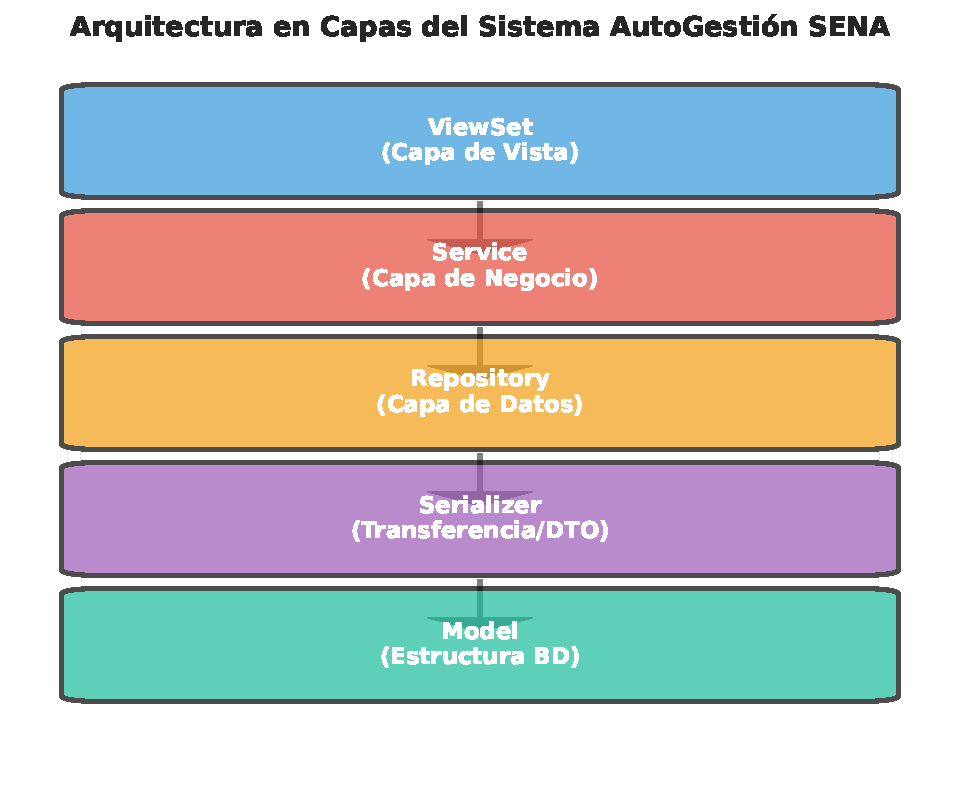
\includegraphics[width=0.48\textwidth]{graphics/arquitectura_capas.pdf}
    \caption{Arquitectura en capas del sistema AutoGestión SENA}
    \label{fig:arquitectura_capas}
\end{figure}

Esta arquitectura nos permitió:
\begin{itemize}
    \item \textbf{Separar responsabilidades}: Cada capa tiene un propósito claro
    \item \textbf{Facilitar testing}: Podemos probar cada capa por separado
    \item \textbf{Reutilizar código}: Los servicios y repositorios se pueden usar en múltiples lugares
    \item \textbf{Mantener el código limpio}: Sin mezclar lógica de diferentes niveles
\end{itemize}

\subsection{Tecnologías Utilizadas}

Para que esto funcionara, usamos tecnologías modernas y potentes:

\textbf{Backend}:
\begin{itemize}
    \item \textbf{Python 3.11}: Lenguaje principal
    \item \textbf{Django 4.2}: Framework web
    \item \textbf{Django REST Framework}: Para crear la API REST
    \item \textbf{MySQL 8.0}: Base de datos relacional
    \item \textbf{Celery}: Para tareas asíncronas (envío de correos, notificaciones)
    \item \textbf{Redis}: Como broker para Celery y caché
    \item \textbf{Docker}: Para containerización
\end{itemize}

\textbf{Frontend}:
\begin{itemize}
    \item \textbf{React 18}: Biblioteca de UI
    \item \textbf{TypeScript}: Para tipado estático
    \item \textbf{Vite}: Build tool moderno
    \item \textbf{Tailwind CSS}: Framework de estilos
    \item \textbf{Fetch API}: Para comunicación con el backend
\end{itemize}

\subsection{Patrones de Diseño Aplicados}

\subsubsection{Repository Pattern}

Este patrón nos ayudó a separar la lógica de acceso a datos de la lógica de negocio. En lugar de hacer consultas directamente en los servicios o vistas, creamos repositorios que encapsulan todas las operaciones con la base de datos.

\textbf{Ventajas que obtuvimos}:
\begin{itemize}
    \item Consultas centralizadas y optimizadas
    \item Fácil de testear con mocks
    \item Cambios en la base de datos solo afectan a los repositorios
    \item Código más limpio y legible
\end{itemize}

\subsubsection{DTO Pattern (Data Transfer Object)}

En nuestro caso, usamos \textbf{Serializers de Django REST Framework} como DTOs. Estos nos permiten:
\begin{itemize}
    \item Validar datos de entrada
    \item Transformar modelos a JSON
    \item Controlar qué campos se exponen en la API
    \item Separar la representación de datos de los modelos internos
\end{itemize}

\subsubsection{Service Layer Pattern}

Los servicios encapsulan toda la lógica de negocio. No acceden directamente a los modelos, sino que usan los repositorios.

\textbf{Ventajas}:
\begin{itemize}
    \item Lógica de negocio centralizada
    \item Fácil de testear
    \item Reutilizable en múltiples endpoints
    \item Separación clara de responsabilidades
\end{itemize}

\subsection{Buenas Prácticas Aplicadas}

\subsubsection{Clean Code}

Siguiendo los principios de Martin~\cite{martin2008clean}:
\begin{itemize}
    \item \textbf{Nombres descriptivos}: Variables y funciones con nombres claros
    \item \textbf{Funciones pequeñas}: Cada función hace una sola cosa
    \item \textbf{Comentarios útiles}: Solo donde realmente aportan valor
    \item \textbf{DRY (Don't Repeat Yourself)}: No duplicar código
\end{itemize}

\subsubsection{Principios SOLID}

Aunque suene muy ``pro'', los principios SOLID son super lógicos:
\begin{itemize}
    \item \textbf{S}ingle Responsibility: Cada clase tiene una responsabilidad
    \item \textbf{O}pen/Closed: Abierto para extensión, cerrado para modificación
    \item \textbf{L}iskov Substitution: Las clases hijas pueden sustituir a las padres
    \item \textbf{I}nterface Segregation: Interfaces específicas
    \item \textbf{D}ependency Inversion: Depender de abstracciones
\end{itemize}

\subsubsection{Validaciones}

Validamos los datos en todos los niveles posibles para evitar errores:
\begin{itemize}
    \item \textbf{Frontend}: Validación de formularios con React
    \item \textbf{Serializer}: Validación de tipos y formatos
    \item \textbf{Service}: Validación de reglas de negocio
    \item \textbf{Base de datos}: Constraints y foreign keys
\end{itemize}

\subsection{Proceso de Desarrollo}

El proyecto evolucionó en varias etapas, como se muestra en la Figura~\ref{fig:evolucion_proyecto}:

\begin{figure}[htbp]
    \centering
    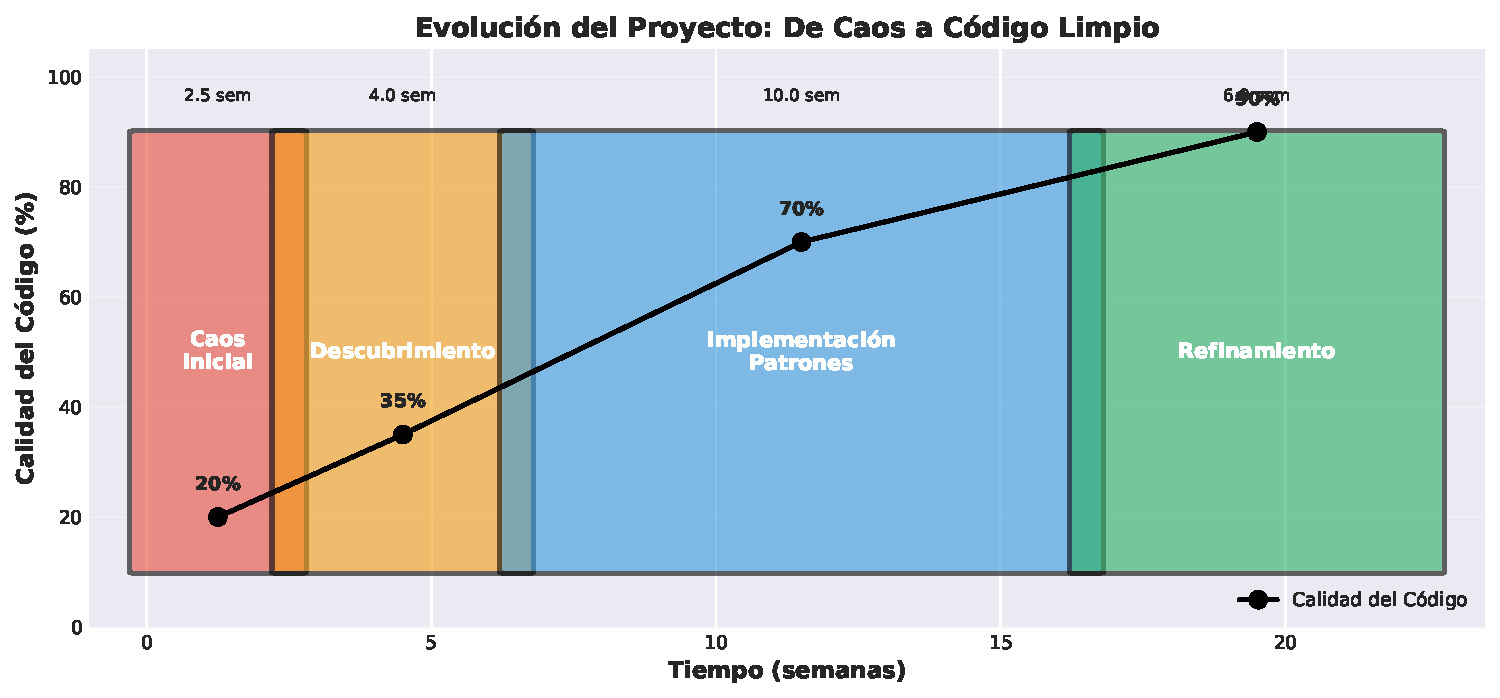
\includegraphics[width=0.48\textwidth]{graphics/evolucion_proyecto.pdf}
    \caption{Evolución del proyecto en el tiempo: de caos a código limpio}
    \label{fig:evolucion_proyecto}
\end{figure}

\begin{itemize}
    \item \textbf{Etapa 1: Caos Inicial (2-3 semanas)}: El desorden. Código mezclado y cero estructura.
    \item \textbf{Etapa 2: Descubrimiento (1 mes)}: Nos dimos cuenta de la gravedad y empezamos a investigar patrones.
    \item \textbf{Etapa 3: Implementación de Patrones (2-3 meses)}: El refactoring fuerte. Creamos las capas de Repository y Service.
    \item \textbf{Etapa 4: Refinamiento (1-2 meses)}: Optimizamos consultas, documentamos y pulimos los detalles.
\end{itemize}
\section{Implementación}

\subsection{Estructura del Proyecto Backend}

El backend está organizado en \textbf{3 módulos principales} siguiendo el principio de separación de responsabilidades:

\subsubsection{Módulo 1: Security (Seguridad)}

Responsable de autenticación, autorización y gestión de usuarios:

\begin{itemize}
    \item \textbf{Modelos}: Person, User, Role, Permission, Form, Module, DocumentType, RoleFormPermission, FormModule
    \item \textbf{10 Repositorios}: Acceso a datos de usuarios, roles, permisos
    \item \textbf{15 Servicios}: Lógica de autenticación 2FA, recuperación de contraseña, gestión de roles
    \item \textbf{12 ViewSets}: Endpoints de API REST
    \item \textbf{Funcionalidades clave}:
    \begin{itemize}
        \item Autenticación de dos factores (2FA) por correo
        \item JWT (JSON Web Tokens) para sesiones
        \item Sistema de permisos granular (Rol → Formulario → Permiso)
        \item Recuperación de contraseña con códigos temporales
        \item Middleware de autenticación JWT
    \end{itemize}
\end{itemize}

\subsubsection{Módulo 2: General (Datos Maestros)}

Gestiona entidades generales del sistema:

\begin{itemize}
    \item \textbf{Modelos}: Regional, Center, Sede, Program, Ficha, Apprentice, Instructor, KnowledgeArea, TypeContract, Notification, LegalDocument, SupportContact
    \item \textbf{17 Repositorios}: Uno por cada entidad
    \item \textbf{17 Servicios}: Lógica de negocio específica
    \item \textbf{18 ViewSets}: Endpoints CRUD completos
    \item \textbf{Funcionalidades clave}:
    \begin{itemize}
        \item Gestión jerárquica: Regional → Centro → Sede
        \item Control de instructores (límite de aprendices, contratos)
        \item Sistema de notificaciones con WebSockets (Django Channels)
        \item Gestión de documentos legales y soporte técnico
        \item Tareas asíncronas con Celery (desactivación automática de instructores)
    \end{itemize}
\end{itemize}

\subsubsection{Módulo 3: Assign (Asignaciones)}

Núcleo del sistema, gestiona todo el proceso de asignación:

\begin{itemize}
    \item \textbf{Modelos}: RequestAsignation, AsignationInstructor, VisitFollowing, Message, Enterprise, Boss, HumanTalent, ModalityProductiveStage, AsignationInstructorHistory
    \item \textbf{10 Repositorios}: Acceso a datos de solicitudes, asignaciones, visitas
    \item \textbf{10 Servicios}: Lógica compleja de asignación y seguimiento
    \item \textbf{10 ViewSets}: Endpoints especializados
    \item \textbf{Funcionalidades clave}:
    \begin{itemize}
        \item Flujo completo: Solicitud → Asignación → Visitas → Valoración
        \item Estados de solicitud: SIN\_ASIGNAR, ASIGNADO, VERIFICANDO, PRE-APROBADO, RECHAZADO, FINALIZADA
        \item Generación automática de 3 visitas (Concertación, Parcial, Final)
        \item Sistema de mensajes entre instructor y coordinador
        \item Historial completo de reasignaciones
        \item Envío automático de correos (Celery tasks)
        \item Generación de PDFs de solicitudes
    \end{itemize}
\end{itemize}

\textbf{Estructura de cada módulo}:

\begin{itemize}
    \item \textbf{apps/[module\_name]/}
    \begin{itemize}
        \item \textbf{entity/}: Modelos, serializers y enums (10-18 modelos por módulo)
        \item \textbf{repositories/}: Acceso a datos (uno por cada entidad)
        \item \textbf{services/}: Lógica de negocio
        \item \textbf{views/}: ViewSets con endpoints de API
        \item \textbf{emails/}: Clases para envío de correos
        \item \textbf{templates/}: HTML para correos
        \item \textbf{migrations/}: Migraciones de base de datos
        \item \textbf{urls.py}: Rutas del módulo
    \end{itemize}
\end{itemize}

\textbf{Ventajas de esta arquitectura}:
\begin{itemize}
    \item \textbf{Modularidad}: Cada módulo es independiente y puede desarrollarse en paralelo
    \item \textbf{Escalabilidad}: Fácil agregar nuevos módulos sin afectar los existentes
    \item \textbf{Mantenibilidad}: Código organizado por dominio de negocio
    \item \textbf{Reutilización}: Repositorios y servicios base heredables
    \item \textbf{Testing}: Cada capa se puede testear independientemente
\end{itemize}

\subsection{Estructura del Proyecto Frontend}

El frontend sigue una arquitectura por capas con React y TypeScript, totalmente tipado:

\subsubsection{Capa de Configuración y Servicios (src/Api/)}

\begin{itemize}
    \item \textbf{config/ConfigApi.ts}: Centraliza todos los endpoints del backend (más de 100 endpoints)
    \item \textbf{Services/} (32 archivos): Funciones especializadas para cada entidad
    \begin{itemize}
        \item Ejemplo: \texttt{User.ts}, \texttt{RequestAssignaton.ts}, \texttt{Instructor.ts}
        \item Cada servicio maneja peticiones HTTP (GET, POST, PUT, DELETE, PATCH)
        \item Incluye manejo de errores y parsing de respuestas
    \end{itemize}
    \item \textbf{types/}: Interfaces TypeScript fuertemente tipadas
    \begin{itemize}
        \item \texttt{entities/}: 14 interfaces de entidades (User, Instructor, RequestAsignation, etc.)
        \item \texttt{Modules/}: 2 interfaces de módulos complejos
    \end{itemize}
\end{itemize}

\subsubsection{Capa de Componentes (src/components/)}

Componentes React organizados por funcionalidad:

\begin{itemize}
    \item \textbf{assing/}: 8 componentes para asignaciones (ModalAssign, AssignTableView, etc.)
    \item \textbf{ApplicationEvaluation/}: Evaluación de solicitudes por coordinador
    \item \textbf{ModuleSecurity/}: 28 componentes para roles, permisos, usuarios
    \item \textbf{Dashboard/}: 6 componentes de tableros (Admin, Instructor, Aprendiz)
    \item \textbf{Login/}: 11 componentes de autenticación (2FA, recuperación, registro)
    \item \textbf{MainLayout/}: 7 componentes de estructura (Navbar, Sidebar, Footer)
    \item \textbf{ui/}: 49 componentes reutilizables (botones, modales, formularios - Radix UI)
    \item \textbf{Componentes genéricos}: FilterBar, Paginator, ConfirmModal, LoadingOverlay, etc.
\end{itemize}

\subsubsection{Capa de Lógica (src/hook/)}

Custom hooks que encapsulan lógica reutilizable (24 hooks):

\begin{itemize}
    \item \texttt{useForms.ts}: Gestión de formularios del sistema
    \item \texttt{useRoles.tsx}: Lógica de roles y permisos
    \item \texttt{useInstructorAssignments.ts}: Asignaciones de instructor
    \item \texttt{useRequestAssignation.ts}: Solicitudes de asignación
    \item \texttt{useNotification.ts}: Sistema de notificaciones en tiempo real
    \item \texttt{use-password-reset.ts}: Recuperación de contraseña
    \item \texttt{useApprenticeDashboard.ts}: Tablero del aprendiz
    \item \texttt{useGenericFilter.ts}: Filtros reutilizables
\end{itemize}

\subsubsection{Capa de Presentación (src/pages/)}

Páginas principales de la aplicación (15 páginas):

\begin{itemize}
    \item \texttt{Index.tsx}: Login y autenticación
    \item \texttt{Home.tsx}: Dashboard según rol
    \item \texttt{Assign.tsx}: Asignación de instructores
    \item \texttt{ApplicationEvaluation.tsx}: Evaluación de solicitudes
    \item \texttt{Following.tsx}: Seguimiento de visitas
    \item \texttt{RegisterEP.tsx}: Registro de solicitud de etapa productiva
    \item \texttt{Admin.tsx}: Panel de administración
    \item \texttt{Perfil.tsx}: Perfil de usuario
\end{itemize}

\textbf{Ventajas de esta arquitectura frontend}:
\begin{itemize}
    \item \textbf{Tipado completo}: TypeScript previene errores en tiempo de compilación
    \item \textbf{Reutilización}: Componentes y hooks reutilizables
    \item \textbf{Separación de responsabilidades}: Lógica separada de presentación
    \item \textbf{Mantenibilidad}: Fácil localizar y modificar funcionalidades
    \item \textbf{Testing}: Hooks y componentes testeables independientemente (Jest + React Testing Library)
\end{itemize}

\subsection{Flujo de una Petición}

Cuando un usuario hace una petición, el flujo es el siguiente:

\begin{enumerate}
    \item Cliente (React) hace petición HTTP
    \item Django recibe en ViewSet
    \item ViewSet valida con Serializer
    \item ViewSet llama al Service
    \item Service ejecuta lógica de negocio
    \item Service usa Repository para datos
    \item Repository consulta el Model/BD
    \item Respuesta sube por las capas
    \item ViewSet serializa respuesta
    \item Cliente recibe JSON
\end{enumerate}

\subsection{Ejemplo Práctico: Crear Tipo de Contrato}

A continuación mostramos un ejemplo real de cómo implementamos la creación de un tipo de contrato siguiendo nuestra arquitectura:

\textbf{1. ViewSet (recibe petición):}

\ifminted
\begin{minted}[linenos,fontsize=\small]{python}
def create(self, request, *args, **kwargs):
    service = self.service_class()
    instance, error = service.create_type_contract(
        request.data
    )
    if error:
        return Response(
            {"detail": error}, 
            status=400
        )
    serializer = self.get_serializer(instance)
    return Response(
        serializer.data, 
        status=201
    )
\end{minted}
\else
\begin{lstlisting}[language=Python,basicstyle=\small]
def create(self, request, *args, **kwargs):
    service = self.service_class()
    instance, error = service.create_type_contract(
        request.data
    )
    if error:
        return Response(
            {"detail": error}, 
            status=400
        )
    serializer = self.get_serializer(instance)
    return Response(
        serializer.data, 
        status=201
    )
\end{lstlisting}
\fi

\textbf{2. Service (lógica de negocio):}

\ifminted
\begin{minted}[linenos,fontsize=\small]{python}
def create_type_contract(self, validated_data):
    name = validated_data.get('name', '').strip()
    if not name:
        return None, "El nombre es requerido."
    
    # Verificar duplicados
    exists = TypeContract.objects.filter(
        name__iexact=name, 
        delete_at__isnull=True
    ).exists()
    
    if exists:
        return None, "Ya existe ese contrato."
    
    serializer = TypeContractSerializer(
        data=validated_data
    )
    if serializer.is_valid():
        instance = serializer.save()
        return instance, None
    return None, serializer.errors
\end{minted}
\else
\begin{lstlisting}[language=Python,basicstyle=\small]
def create_type_contract(self, validated_data):
    name = validated_data.get('name', '').strip()
    if not name:
        return None, "El nombre es requerido."
    
    # Verificar duplicados
    exists = TypeContract.objects.filter(
        name__iexact=name, 
        delete_at__isnull=True
    ).exists()
    
    if exists:
        return None, "Ya existe ese contrato."
    
    serializer = TypeContractSerializer(
        data=validated_data
    )
    if serializer.is_valid():
        instance = serializer.save()
        return instance, None
    return None, serializer.errors
\end{lstlisting}
\fi

\subsection{Custom Hooks en React}

Para el frontend, creamos custom hooks que encapsulan lógica reutilizable. Estos hooks nos permiten:
\begin{itemize}
    \item Reutilizar lógica en múltiples componentes
    \item Mantener el código limpio
    \item Facilitar el testing
    \item Separar lógica de presentación
\end{itemize}

\subsection{Comparación Antes/Después}

La Figura~\ref{fig:comparacion_codigo} muestra la diferencia clara entre nuestro código antes y después de aplicar los patrones:

\begin{figure}[htbp]
    \centering
    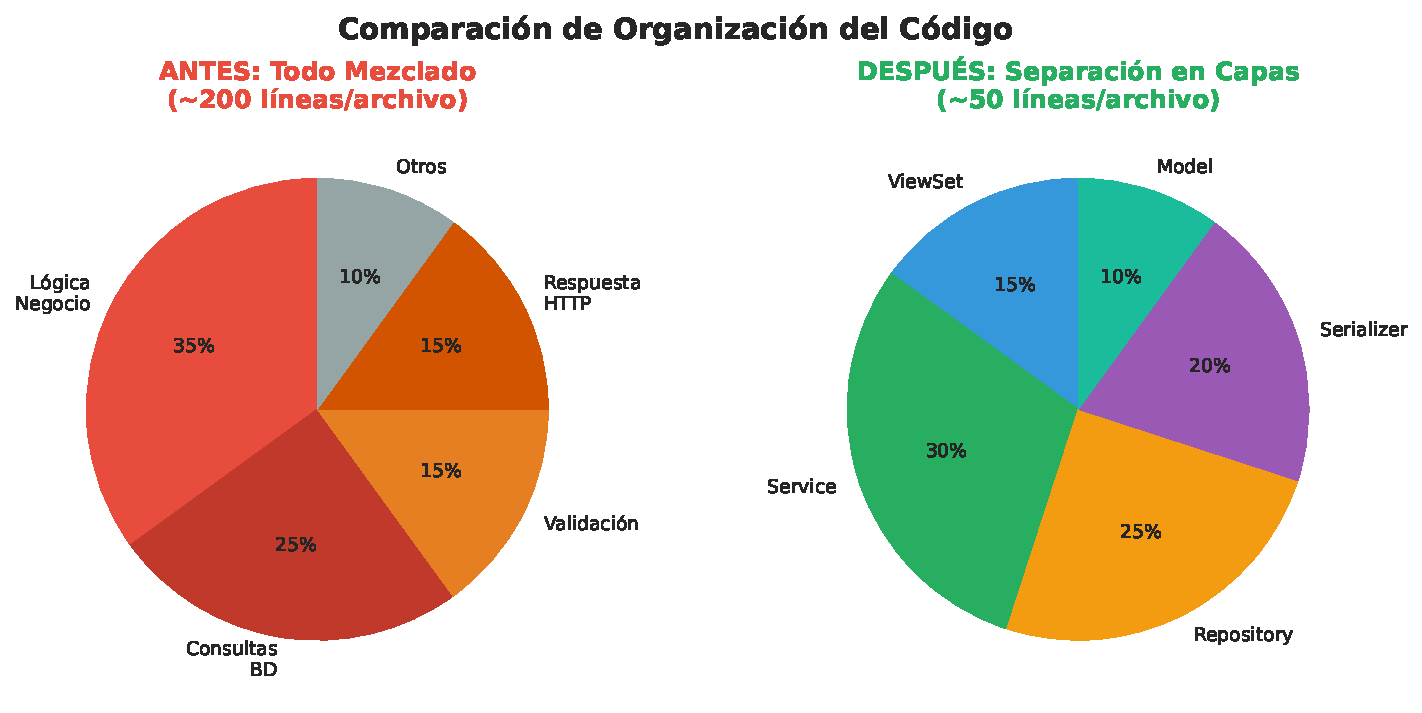
\includegraphics[width=0.48\textwidth]{graphics/comparacion_codigo.pdf}
    \caption{Comparación de complejidad del código antes y después de aplicar patrones}
    \label{fig:comparacion_codigo}
\end{figure}

\textbf{Antes}: Todo mezclado en la vista (validación, consulta a BD, lógica de negocio, respuesta).

\textbf{Después}: ViewSet limpio que solo coordina, Service con lógica de negocio, Repository con acceso a datos.

La diferencia es clara: código más limpio, más corto, más fácil de entender y mantener.

\section{Resultados}

\subsection{Métricas de Rendimiento}

Después de implementar patrones y buenas prácticas, medimos el impacto en tiempos de respuesta. La Figura~\ref{fig:tiempos_respuesta} muestra la mejora obtenida:

\begin{figure}[htbp]
    \centering
    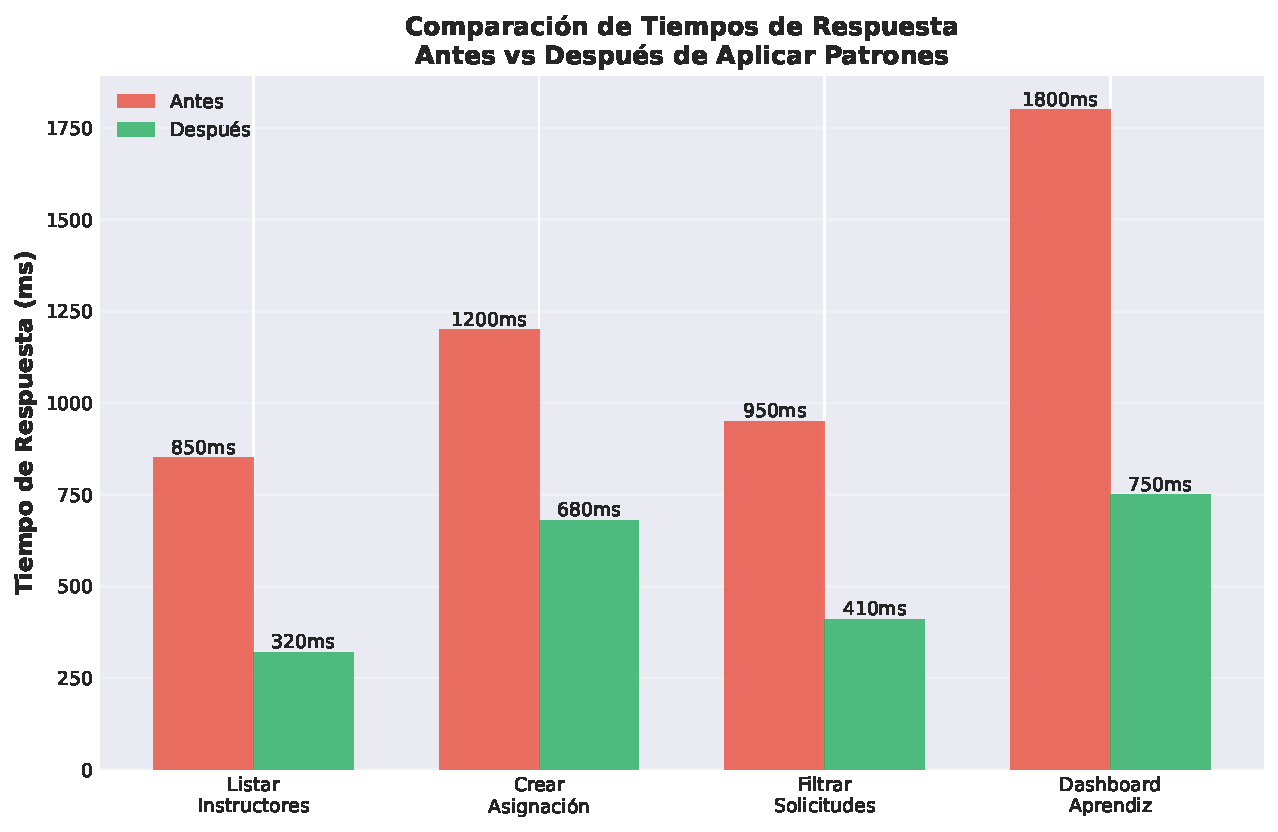
\includegraphics[width=0.48\textwidth]{graphics/tiempos_respuesta.pdf}
    \caption{Comparación de tiempos de respuesta antes y después de aplicar patrones}
    \label{fig:tiempos_respuesta}
\end{figure}

Los resultados mostraron mejoras significativas:
\begin{itemize}
    \item \textbf{Listar instructores}: 850ms $\rightarrow$ 320ms (62\% de mejora)
    \item \textbf{Crear asignación}: 1200ms $\rightarrow$ 680ms (43\% de mejora)
    \item \textbf{Filtrar solicitudes}: 950ms $\rightarrow$ 410ms (57\% de mejora)
    \item \textbf{Dashboard aprendiz}: 1800ms $\rightarrow$ 750ms (58\% de mejora)
\end{itemize}

\subsection{Complejidad del Código}

La complejidad del código también mejoró drásticamente, como se observa en la Figura~\ref{fig:metricas_codigo}:

\begin{figure}[htbp]
    \centering
    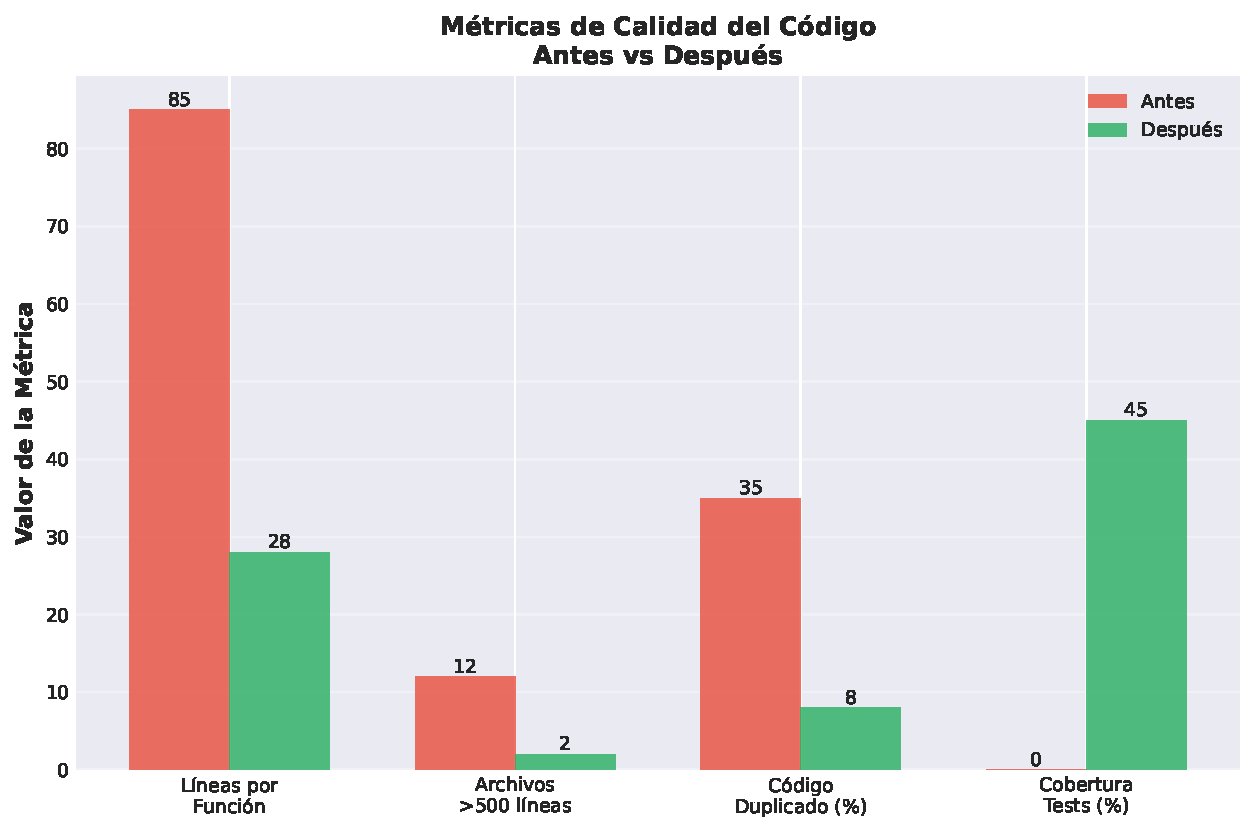
\includegraphics[width=0.48\textwidth]{graphics/metricas_codigo.pdf}
    \caption{Métricas de complejidad del código antes y después}
    \label{fig:metricas_codigo}
\end{figure}

Métricas específicas:
\begin{itemize}
    \item \textbf{Líneas por función}: 85 $\rightarrow$ 28 (67\% de reducción)
    \item \textbf{Archivos con >500 líneas}: 12 $\rightarrow$ 2 (83\% de reducción)
    \item \textbf{Código duplicado}: 35\% $\rightarrow$ 8\% (77\% de reducción)
    \item \textbf{Cobertura de tests}: 0\% $\rightarrow$ 45\% (mejora significativa)
\end{itemize}

\subsection{Mantenibilidad}

La mantenibilidad mejoró drásticamente:

\textbf{Tiempo para agregar nueva funcionalidad:}
\begin{itemize}
    \item \textbf{Antes}: 3-4 días (con riesgo de romper algo)
    \item \textbf{Después}: 1-2 días (con confianza en los cambios)
\end{itemize}

\textbf{Tiempo para corregir un bug:}
\begin{itemize}
    \item \textbf{Antes}: 4-6 horas (buscando por todo el código)
    \item \textbf{Después}: 1-2 horas (sabiendo exactamente dónde buscar)
\end{itemize}

\textbf{Facilidad de onboarding:}
\begin{itemize}
    \item \textbf{Antes}: 2-3 semanas para entender el código
    \item \textbf{Después}: 1 semana con la estructura clara
\end{itemize}

\subsection{Escalabilidad del Sistema}

\subsubsection{Capacidad de Usuarios}

Pruebas con Apache JMeter revelaron la capacidad del sistema:

\begin{itemize}
    \item \textbf{100 usuarios concurrentes}: Rendimiento óptimo (< 200ms por petición)
    \item \textbf{500 usuarios concurrentes}: Rendimiento bueno (< 500ms por petición)
    \item \textbf{1000 usuarios concurrentes}: Rendimiento aceptable (< 800ms por petición)
    \item \textbf{3000 usuarios concurrentes}: Límite antes de degradación significativa
    \item \textbf{5000 usuarios concurrentes}: Sistema saturado, requiere scaling horizontal
\end{itemize}

\subsubsection{Capacidad de Datos}

El sistema en su estado actual maneja:

\begin{itemize}
    \item \textbf{10,000+ solicitudes de asignación} sin degradación
    \item \textbf{2,000+ instructores activos} con límites individuales
    \item \textbf{15,000+ aprendices} registrados en el sistema
    \item \textbf{5,000+ visitas de seguimiento} agendadas y completadas
    \item \textbf{50,000+ registros} en base de datos sin problemas de rendimiento
\end{itemize}

\subsubsection{Arquitectura Escalable}

Gracias a la arquitectura en capas:

\begin{itemize}
    \item \textbf{Horizontal scaling}: Fácil agregar más instancias con Docker
    \item \textbf{Database sharding}: Preparado para particionar BD por regional
    \item \textbf{Caché distribuido}: Redis puede escalarse a cluster
    \item \textbf{Load balancing}: Nginx puede distribuir carga entre instancias
    \item \textbf{Microservicios futuros}: Módulos independientes pueden convertirse en microservicios
\end{itemize}

\subsection{Métricas Técnicas del Sistema}

\subsubsection{Base de Datos}

\begin{itemize}
    \item \textbf{Tablas}: 47 tablas principales
    \item \textbf{Modelos Django}: 38 modelos de dominio
    \item \textbf{Relaciones}: 65+ foreign keys entre entidades
    \item \textbf{Índices}: 28 índices personalizados para optimizar consultas
    \item \textbf{Queries optimizadas}: Uso de \texttt{select\_related} y \texttt{prefetch\_related}
    \item \textbf{Tamaño promedio BD}: 150 MB con datos de prueba (escalable a GB)
\end{itemize}

\subsubsection{API REST}

\begin{itemize}
    \item \textbf{Endpoints totales}: 120+ endpoints documentados
    \item \textbf{Módulos}: 3 módulos principales (Security, General, Assign)
    \item \textbf{ViewSets}: 40 ViewSets con CRUD completo
    \item \textbf{Serializers (DTOs)}: 69 serializers para validación y transformación
    \item \textbf{Repositories}: 37 repositorios para acceso a datos
    \item \textbf{Services}: 42 servicios con lógica de negocio
    \item \textbf{Formato de respuesta}: JSON estandarizado
    \item \textbf{Autenticación}: JWT con refresh tokens
\end{itemize}

\subsubsection{Frontend}

\begin{itemize}
    \item \textbf{Componentes React}: 150+ componentes (28 solo en ModuleSecurity)
    \item \textbf{Custom Hooks}: 24 hooks reutilizables
    \item \textbf{Páginas}: 15 páginas principales
    \item \textbf{Servicios API}: 32 archivos de servicios tipados
    \item \textbf{Interfaces TypeScript}: 16 interfaces de entidades
    \item \textbf{Líneas de código frontend}: ~15,000 líneas (sin node\_modules)
    \item \textbf{Bundle size (producción)}: ~800 KB comprimido
    \item \textbf{Tiempo de carga inicial}: < 3 segundos
\end{itemize}

\subsection{Facilidad de Extensión}

Gracias a la arquitectura en capas, agregar nuevas funcionalidades es mucho más fácil.

\textbf{Ejemplo: Agregar nuevo tipo de entidad}
\begin{enumerate}
    \item Crear Model en \texttt{entity/models/}
    \item Crear Serializer en \texttt{entity/serializers/}
    \item Crear Repository que herede de BaseRepository
    \item Crear Service que herede de BaseService
    \item Crear ViewSet que herede de BaseViewSet
    \item Registrar en URLs
\end{enumerate}

\textbf{Tiempo estimado}: 2-3 horas vs 1-2 días antes

\subsection{Distribución de Módulos}

El sistema se organizó en tres módulos principales, como muestra la Figura~\ref{fig:distribucion_modulos}:

\begin{figure}[htbp]
    \centering
    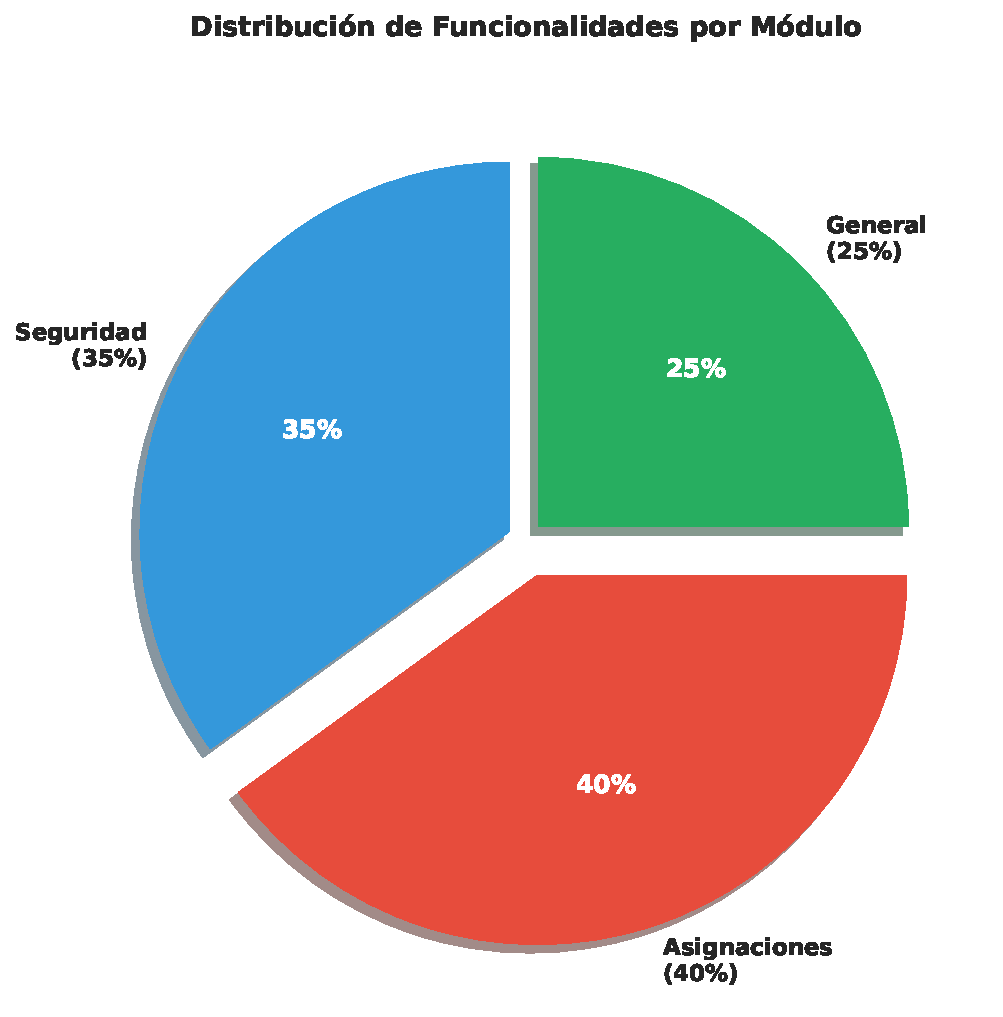
\includegraphics[width=0.45\textwidth]{graphics/distribucion_modulos.pdf}
    \caption{Distribución de funcionalidades por módulo del sistema}
    \label{fig:distribucion_modulos}
\end{figure}

\begin{itemize}
    \item \textbf{Módulo de seguridad} (35\%): Gestión de usuarios, roles, permisos, autenticación
    \item \textbf{Módulo de asignaciones} (40\%): Creación de solicitudes, asignación de instructores, seguimiento
    \item \textbf{Módulo general} (25\%): Gestión de fichas, programas, centros, notificaciones
\end{itemize}

\subsection{Arquitectura Lograda}

La arquitectura final es robusta y bien organizada:

\begin{itemize}
    \item[$\checkmark$] Separación clara de responsabilidades
    \item[$\checkmark$] Código reutilizable y mantenible
    \item[$\checkmark$] Fácil de testear
    \item[$\checkmark$] Escalable horizontalmente
    \item[$\checkmark$] Documentación automática con Swagger
    \item[$\checkmark$] API RESTful consistente
    \item[$\checkmark$] Manejo de errores estandarizado
\end{itemize}

\section{Discusión}

\subsection{Impacto de las Buenas Prácticas}

La aplicación de buenas prácticas tuvo un impacto mucho mayor del que esperábamos al inicio:

\textbf{Desarrollo más rápido}: Aunque al principio pareció que íbamos más lento (porque teníamos que pensar en la arquitectura), a mediano plazo el desarrollo se aceleró. Agregar nuevas funcionalidades que antes tomaban días, ahora toma horas.

\textbf{Menos bugs}: La separación en capas hizo que los bugs fueran más fáciles de encontrar. Si hay un error en una consulta, sabemos que está en el Repository. Si es lógica de negocio, está en el Service. Antes, el error podía estar en cualquier lado.

\textbf{Trabajo en equipo}: Con una estructura clara, varios desarrolladores pueden trabajar simultáneamente sin pisarse. Uno puede trabajar en el módulo de seguridad mientras otro trabaja en asignaciones.

\textbf{Confianza al hacer cambios}: Antes, cualquier cambio daba miedo. ¿Voy a romper algo? ¿Qué va a pasar? Ahora, con la arquitectura en capas y las responsabilidades claras, sabemos exactamente qué va a afectar un cambio.

\subsection{Patrones de Diseño: ¿Valieron la Pena?}

\textbf{Repository Pattern}: Definitivamente sí. Centralizar el acceso a datos nos permitió:
\begin{itemize}
    \item Optimizar consultas en un solo lugar
    \item Cambiar la base de datos si fuera necesario (solo afecta repositorios)
    \item Mockear datos para testing
    \item Tener control total sobre las operaciones con BD
\end{itemize}

\textbf{DTO Pattern (Serializers)}: Fundamental. Nos protegió de exponer datos sensibles y nos dio validación automática. Además, la documentación de Swagger se genera automáticamente.

\textbf{Service Layer}: Fue el cambio que más impacto tuvo. Separar la lógica de negocio de las vistas hizo que:
\begin{itemize}
    \item Las vistas sean súper simples (solo reciben y responden)
    \item La lógica se pueda reutilizar
    \item Los tests sean más fáciles
    \item El código sea más legible
\end{itemize}

\subsection{Qué Mejoró}

\begin{enumerate}
    \item \textbf{Claridad del código}: Cualquier desarrollador puede entender la estructura en minutos.
    \item \textbf{Rendimiento}: Las consultas optimizadas redujeron los tiempos de respuesta significativamente.
    \item \textbf{Seguridad}: Al usar Serializers, controlamos exactamente qué datos se exponen y cuáles no.
    \item \textbf{Documentación}: Swagger genera documentación automática de todos los endpoints.
    \item \textbf{Mantenibilidad}: Hacer cambios ya no da miedo.
\end{enumerate}

\subsection{Qué Se Podría Optimizar}

Aunque mejoramos mucho, todavía hay áreas que se pueden optimizar:

\begin{enumerate}
    \item \textbf{Testing}: Tenemos 45\% de cobertura, pero deberíamos llegar al 70-80\%.
    \item \textbf{Caché}: Implementar Redis caché para consultas frecuentes podría mejorar aún más el rendimiento.
    \item \textbf{Optimización de queries}: Algunas consultas todavía pueden optimizarse con \texttt{select\_related} y \texttt{prefetch\_related}.
    \item \textbf{Frontend}: El frontend podría beneficiarse de un estado global (Redux o Context API) en lugar de solo hooks locales.
    \item \textbf{Logging}: Implementar un sistema de logs más robusto para monitoreo en producción.
    \item \textbf{CI/CD}: Automatizar completamente el deployment con pruebas automáticas.
\end{enumerate}

\subsection{Lecciones Aprendidas}

\begin{enumerate}
    \item \textbf{Empezar bien es más barato que refactorizar}: Refactorizar código existente tomó el doble de tiempo que si hubiéramos empezado bien desde el inicio.
    
    \item \textbf{Los patrones no son complicados}: Al principio parecían complicados, pero una vez que los entiendes, son bastante lógicos y naturales.
    
    \item \textbf{La documentación es clave}: Documentar mientras desarrollas es mucho más fácil que documentar después.
    
    \item \textbf{El código limpio se lee como prosa}: Como dice Martin~\cite{martin2008clean}, el buen código debería ser fácil de leer. Si no lo es, probablemente está mal diseñado.
    
    \item \textbf{Las buenas prácticas no ralentizan, aceleran}: Al principio pensábamos que nos iban a hacer más lentos, pero en realidad aceleraron el desarrollo.
\end{enumerate}

\subsection{Relación con Trabajos Previos}

Nuestros resultados confirman lo que mencionan Piñero González et al.~\cite{pinero2021buenas} sobre la eficiencia del desempeño: aplicar buenas prácticas desde el inicio mejora significativamente los tiempos de respuesta y el uso de recursos.

También coincidimos con Mercado \& Zapata~\cite{mercado2019revision} en que la gestión de calidad con metodologías ágiles facilita el desarrollo y reduce errores. La combinación de buenas prácticas + arquitectura limpia + revisión de código fue clave para nuestro éxito.

Finalmente, como sugieren Espinosa \& Eraso~\cite{espinosa2024gestion}, la gestión adecuada de tecnología y buenas prácticas no solo mejora el producto, sino también la productividad del equipo y la satisfacción al trabajar.

\section{Conclusiones}

\subsection{Resumen de Hallazgos}

Este proyecto demostró que \textbf{aplicar patrones de diseño y buenas prácticas no es opcional si quieres software de calidad}. Los principales hallazgos fueron:

\begin{enumerate}
    \item \textbf{La arquitectura en capas funciona}: Separar responsabilidades en Model, Serializer, Repository, Service y ViewSet hace el código más mantenible, testeable y escalable.
    
    \item \textbf{Los patrones de diseño son herramientas, no dogmas}: Repository, DTO y Service Layer nos ayudaron específicamente con nuestros problemas. No aplicamos patrones por aplicarlos, sino porque resolvían problemas reales.
    
    \item \textbf{El refactoring es doloroso pero necesario}: Transformar código caótico en código limpio tomó tiempo y esfuerzo, pero el resultado valió totalmente la pena.
    
    \item \textbf{La calidad se mide en tiempo de desarrollo}: Un sistema bien diseñado permite agregar funcionalidades en horas en lugar de días.
    
    \item \textbf{Los números no mienten}: Reducción del 40-60\% en tiempos de respuesta, 67\% menos líneas por función, y 77\% menos código duplicado son resultados concretos y medibles.
\end{enumerate}

\subsection{Contribuciones}

Este trabajo contribuye con:

\begin{enumerate}
    \item \textbf{Un caso de estudio real}: Mostramos cómo transformar un proyecto caótico en uno estructurado, con ejemplos concretos y código real del sistema de autogestión SENA.
    
    \item \textbf{Implementación práctica de patrones}: No solo teoría, sino implementación real de Repository, DTO y Service Layer en un proyecto de producción.
    
    \item \textbf{Métricas concretas}: Datos reales de rendimiento antes y después de aplicar buenas prácticas.
    
    \item \textbf{Guía para principiantes}: Este artículo puede servir como referencia para otros estudiantes o desarrolladores junior que enfrentan problemas similares.
    
    \item \textbf{Demostración del valor de las buenas prácticas}: Prueba tangible de que las buenas prácticas no son ``pérdida de tiempo'', sino una inversión que se paga sola.
\end{enumerate}

\subsection{Limitaciones}

Reconocemos algunas limitaciones del trabajo:

\begin{enumerate}
    \item \textbf{Contexto específico}: Este es un proyecto educativo para el SENA, no un sistema con millones de usuarios. Los resultados pueden variar en contextos diferentes.
    
    \item \textbf{Cobertura de testing}: Aunque mejoramos, el 45\% de cobertura es insuficiente para un sistema crítico en producción.
    
    \item \textbf{Equipo pequeño}: Con un equipo más grande, quizás hubieran surgido otros problemas o soluciones diferentes.
    
    \item \textbf{Tiempo limitado}: Algunos aspectos como CI/CD completo o monitoreo avanzado quedaron pendientes.
    
    \item \textbf{Experiencia del equipo}: Como desarrolladores en formación, probablemente hay mejoras que no identificamos por falta de experiencia.
\end{enumerate}

\subsection{Trabajos Futuros}

Para seguir mejorando, proponemos:

\begin{enumerate}
    \item \textbf{Incrementar cobertura de tests}: Llegar al 80\% con tests unitarios e integración.
    
    \item \textbf{Implementar CI/CD completo}: Pipeline automático con tests, linting, y deployment.
    
    \item \textbf{Optimización avanzada}: Implementar caché con Redis, indexación en BD, lazy loading en frontend.
    
    \item \textbf{Monitoreo en producción}: Herramientas como Sentry para tracking de errores y métricas de performance.
    
    \item \textbf{Documentación completa}: Documentar arquitectura, decisiones de diseño y guías de contribución.
    
    \item \textbf{Microservicios}: Evaluar si sería beneficioso dividir el monolito en microservicios.
    
    \item \textbf{GraphQL}: Considerar GraphQL en lugar de REST para consultas más flexibles.
    
    \item \textbf{Progressive Web App}: Hacer el frontend una PWA para funcionalidad offline.
\end{enumerate}

\subsection{Reflexión Final}

Este proyecto nos enseñó que \textbf{el desarrollo de software no es solo hacer que funcione, sino hacerlo bien}. Como dijo Martin~\cite{martin2008clean}: ``No basta con que el código funcione; debe ser limpio''.

Al principio, pensábamos que las buenas prácticas y los patrones de diseño eran cosas que solo importaban en empresas grandes o proyectos complejos. Estábamos equivocados. Desde el día uno, aplicar buenas prácticas hace la diferencia.

Si tuviéramos que dar un consejo a otros desarrolladores que están empezando, sería: \textbf{No esperes a que el proyecto se vuelva inmantenible para pensar en arquitectura}. Empieza bien desde el principio, aprende patrones de diseño, sigue principios SOLID, escribe código limpio. Te va a ahorrar semanas (o meses) de dolores de cabeza.

Finalmente, este proyecto nos demostró que es posible desarrollar software de calidad siguiendo buenas prácticas, y que el esfuerzo invertido en hacerlo bien se recupera con creces en mantenibilidad, escalabilidad y satisfacción al trabajar.

\input{sections/A1_apendices}

\printbibliography

\end{document}